\chapter{Kombinatorika, pravdepodobnosť a štatistika}

\section{Kombinatorika}

\begin{example}
	Marta sa oblieka do školy. Chce si obliecť tričko, sukňu a obuť tenisky. V skrini má 3 sukne rôznej dĺžky, 5 tričiek rôznej farby a 4 páry tenisiek z rôzneho matriálu. Koľkými rôznymi spôsobmi sa môže Marta obliecť a obuť? 
\end{example}

\begin{example}
	Patrik mal za úlohu vypísať všetky trojciferné čísla skladájucich sa z cifier 0, 2, 5 a 8 bez opakovania. Podarilo sa mu nájsť tieto čísla: 205, 502, 805, 802, 520, 820, 850, 240. Koľko čísel mu ešte chýba? 
\end{example}

\begin{example}
	Anna si pripravuje na raňajky ovsenú, pohankovú alebo pšeničnú kašu s jedným z troch druhov ovocia ochutenú medom alebo kakaom. Koľko rôznych raňajok si vie pripraviť z uvedených surovín.
	
	\begin{center}
		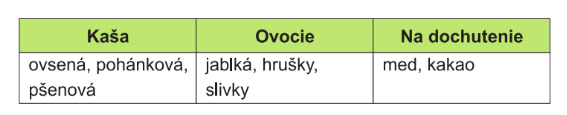
\includegraphics{assets/tab2.png}
	\end{center}
\end{example}

\begin{example}
	Koľko štvorciferných čísel vieme zostrojiť z cifier 3 a 8 tak, aby sa každá cifra vyskytovala práve dvakrát?
\end{example}

\begin{example}
	Koľko dvociferných párnych čísel vieme zostrojiť z cifier 2, 4 a 7? Cifry sa v číslach môžu opakovať.
\end{example}

\begin{example}
	4 kamarátky si kúpili lístky do kina v jednom rade. Koľkými spôsobmi sa vedia usadiť?
\end{example}

\begin{example}
	Týždeň sa Zuzka chystá na prijímacie skúšky na strednú školu v Bratislave. Otecko rozmýšľal, ako sa dostanú z DOMU do Bratislavy. Na internete zistil, že z DOMU do Trnavy môže ísť 3 rôznymi cestami a z Trnavy vedú do Bratislavy 4 rôzne cesty. Koľkými rôznymi spôsobmi sa môže Zuzka s oteckom dostať z DOMU do Bratislavy?
	
\end{example}

\begin{example}
	Na turnaji sa zúčastnilo 8 tímov. Boli rozdelené do dvoch skupín po štyroch. V každej skupine hral každý s každým jedenkrát. Víťaz prvej skupiny si na záver zahral finále s víťazom druhej skupiny. Iné zápasy sa nehrali. Koľko zápasov sa celkovo odohralo na turnaji?
\end{example}

\begin{example}
	Rodičia a ich deti Anna a Boris sa rozhodli stráviť nedeľné poludnie hraním šachu. Pričom mali v pláne hrať jednu partiu šachu každý s každým. Rozhodni, ktorí dvaja spolu neodohrali partiu, ak vieš, že:
	\begin{itemize}
		\item Anna vyhrala nad Borisom.
		\item Otec trikrát remízoval.
		\item Boris má na konte výhru, remízu aj prehru.
	\end{itemize}
	
	Spoločnú partiu neodohrali
	
	\begin{enumerate}
		\item otec a mama.
		\item Anna a otec.
		\item mama a Anna.
		\item Boris a mama.
	\end{enumerate}
\end{example}

\section{Pravdepodobnosť}

\begin{example}
	Monika s Filipom veľmi radi hrávajú spoločenské hry. Keďže dnes vonku pršalo, rozhodli sa, že si jednu vedomostnú hru zahrajú. V hre je spolu 25 kartičiek s otázkami o Slovensku. Filip tvrdil, že na všetky otázky okrem piatich už ovláda odpoveď. Aká je pravdepodobnosť, že si ako prvú vytiahne otázku, ktorú určite vie? Výsledok vyjadri v percentách.
\end{example}

\begin{example}
	Pán Martin má spolu v knižnici 150 kníh. Rozdelil ich do piatich kategórií. Románov je 75, encyklopédií je 5-krát menej ako románov. Detských kníh má o 4 viac ako cestopisov. V kategórií hobby si nechal 20 kníh. \\
	
	Do jednej z kníh z kategórie hobby si pán Martin odložil úspory. Jeho suseda zaujali knihy práve z tejto kategórie a chcel si nejakú z nich požičať. Aká je pravdepodobnosť, že si vyberie práve tú knihu, v ktorej mal pán Martin odložené úspory? Výsledok uveď ako zlomok v základnom tvare.
\end{example}


\begin{example}
	V triede je 20 žiakov. Každý z nich pripravil projekt z geografie. Na hodine vždy vyžrebujú jedného žiaka z tých, ktorí ešte svoj projekt neprezentovali, na prezentovanie na nasledujúcu hodinu. Aká je pravdepodobnosť, že vyberú práve Petra, ak už prezentovalo 13 jeho spolužiakov? Výsledok zapíš ako zlomok v základnom tvare.
\end{example}

\begin{example}
	Počas automatického ladenia TV prijímač vyhľadal 25 kanálov, z toho boli 4 hudobné. Kanály sa do pamäte ukladajú v náhodnom poradí. Vyjadri v percentách pravdepodobnosť, že ako prvý bude uložený hudobný kanál.
\end{example}

\begin{example}
	V nepriehľadnom vrecúšku sú 2 guľôčky biele, dve červené a dve modré. Najmenej koľko guľôčok musíme z vrecúška vytiahnuť, aby sme si boli istí, že sme vytiahli aspoň jednu bielu guľôčku?
\end{example}

\begin{example}
	Zuzana má na svojom mobilnom telefóne 5 priečinkov  srôznymi hudbnými štýlmi. V tabuľke sú uvedené ich názvy a počty skladieb, ktoré obsahujú. Doplnte chýbajúce číslo tak, aby pri funkcii náhodného prehrávania hrala rocková skladba s pravdepodobnosťou 21\% ako prvá. 
	
	\begin{center}
		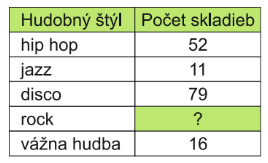
\includegraphics{assets/tab4.png}
	\end{center}
\end{example}

\begin{example}
	Na polici je uložených 27 atlasov, 29 slovníkov, 8 učebníc a 16 encyklopédií. Aká je pravdepodonosť, že náhodne vybratá kniha bude encyklopédia? Výsledok uveď v percentách.
\end{example}

\begin{example}
	V nepriehľadnom vrecúšku sú kocky rôznej farby. 10 je bielych, 10 modrých a 10 červených kociek. Postupne sme vybrali 5 bielych kociek,  3 modré a 2 červené kocky. Aká je pravdepodonosť, že pri ďalšom náhodnom výbere vyberieme ako ďalšú bielu kocku? Výsledok uveď v percentách.
\end{example}

\section{Štatistika}

\begin{example}
	Lenka ušetrila v januári 22 eur, vo februári 16 eur a v marci 21 eur. Koľko eur ušetrila v apríli, ak za tieto 4 mesiace ušetrila v priemere 20 eur mesačne? 
\end{example}

\begin{center}
	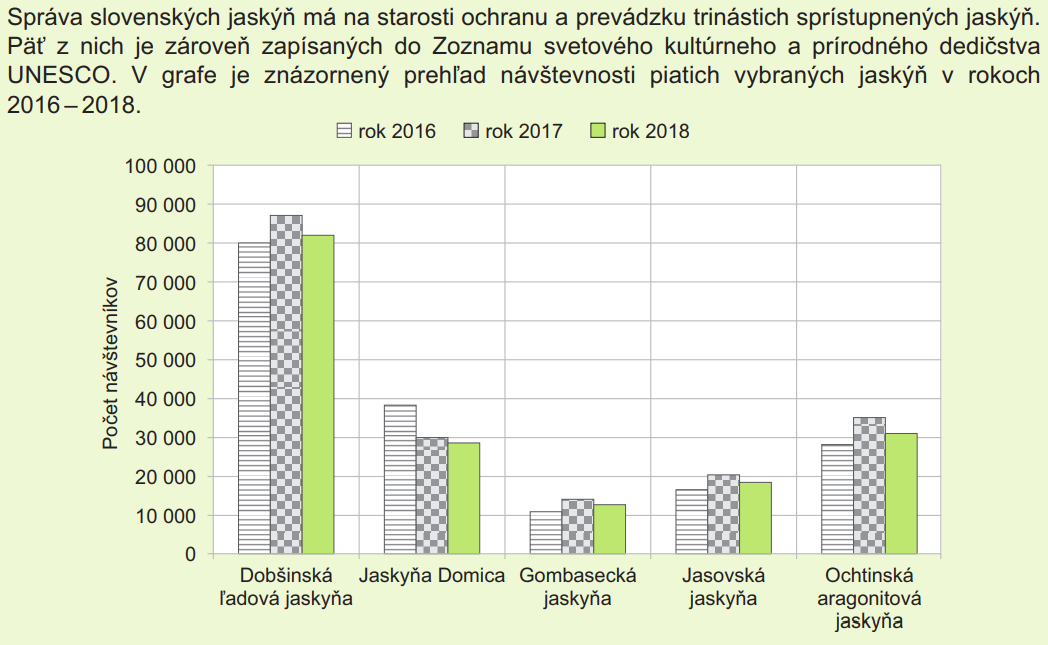
\includegraphics[width=\linewidth]{assets/jaskyne_graf.png}
	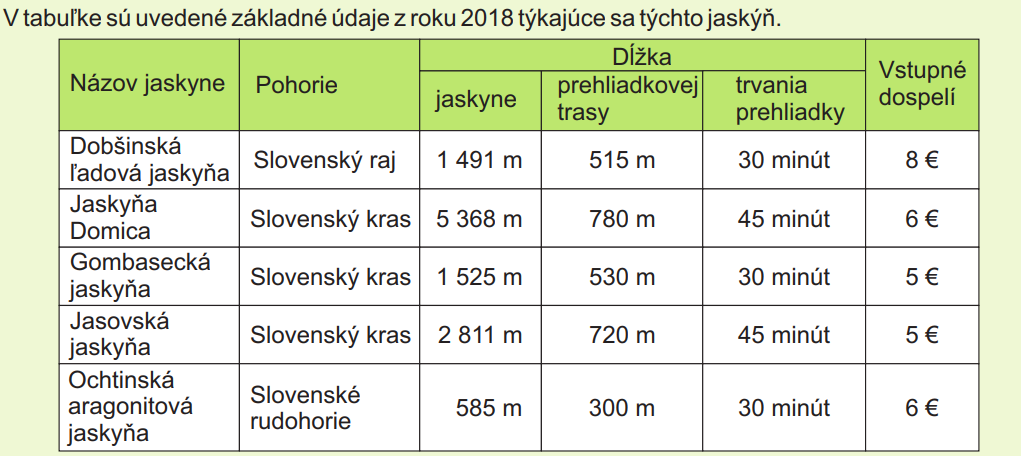
\includegraphics[width=\linewidth]{assets/jaskyne_tab.png}
	
\end{center}

\begin{example}
	Rozhodni o pravdivosti nasledujúcich dvoch tvrdení:
	\begin{enumerate}
		\item Len v jednej z vybraných jaskýň bola návštevnosť v roku 2018 nižšia ako v roku 2016.
		\item Ochtinskú aragonitovú jaskyňu navštívilo počas sledovaného obdobia viac ako 120-tisíc
		návštevníkov
	\end{enumerate}
	
	Možnosti:
	\begin{enumerate}
		\item Iba prvé tvrdenie je pravdivé.
		\item Iba druhé tvrdenie je pravdivé.
		\item Pravdivé sú obe tvrdenia
		\item Pravdivé nie je ani jedno tvrdenie.
	\end{enumerate}
\end{example}

\begin{example}
	V ktorej z vybraných jaskýň návštevník nebol, ak počas prehliadok ostatných štyroch jaskýň nachodil spolu 2 315 m a na vstupnom zaplatil spolu 25 €?
	
	\begin{enumerate}
		\item Dobšinská ľadová jaskyňa
		\item Jaskyňa Domica
		\item Gombasecká jaskyňa
		\item Jasovská jaskyňa
	\end{enumerate}
\end{example}

\begin{example}
	V bytovom dome býva 60 rodín. Kruhový diagram znázorňuje percentuálne zastúpenie počtu podľa počtu áut v rodine. Koľko rodín má najmenej 2 autá?
	
	\begin{center}
		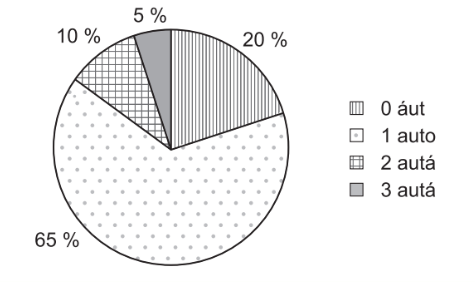
\includegraphics{assets/auta_graf.png}
	\end{center}
\end{example}

\begin{center}
	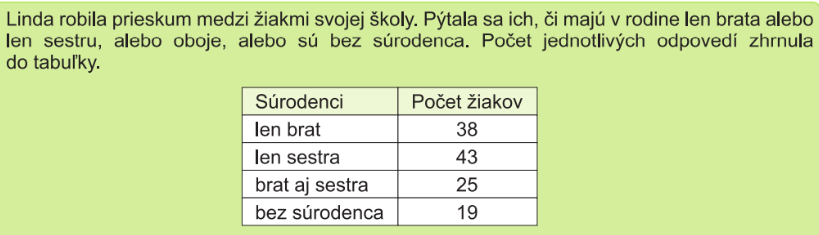
\includegraphics{assets/tab5.png}
\end{center}

\begin{example}
	Posúď pravdivosť nasledujúcich 2 tvrdení:
	
	\begin{itemize}
		\item Linda zistila, že bez súrodenca je viac ako 10\% žiakov.
		\item U pätiny opýtaných žiakov sú určite najmenej tri deti.
	\end{itemize}
	
	Pravdivé
	\begin{enumerate}
		\item je len prvé tvrdenie.
		\item je len druhé trdenie.
		\item nie je žiadne z tvrdení.
		\item sú obe tvrdenia.
	\end{enumerate}
\end{example}

\begin{center}
	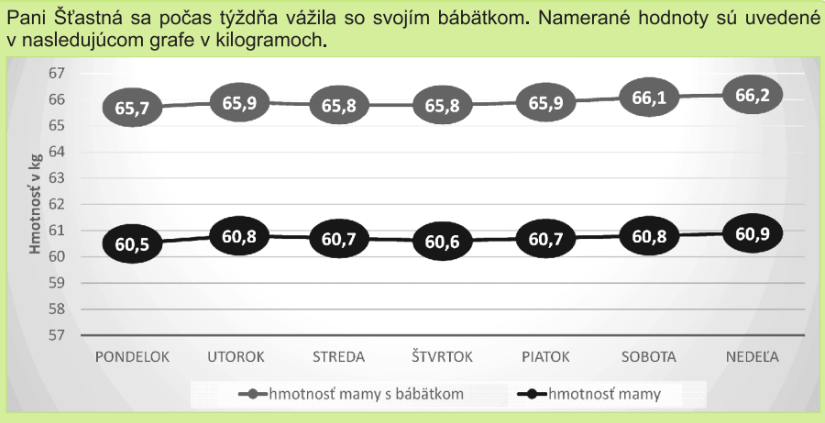
\includegraphics{assets/babatka.png}
\end{center}

\begin{example}
	O koľko kilogramov bola hmotnosť bábätka väčšia v nedeľu ako v pondelok?
\end{example}

\begin{example}
	
	\begin{center}
		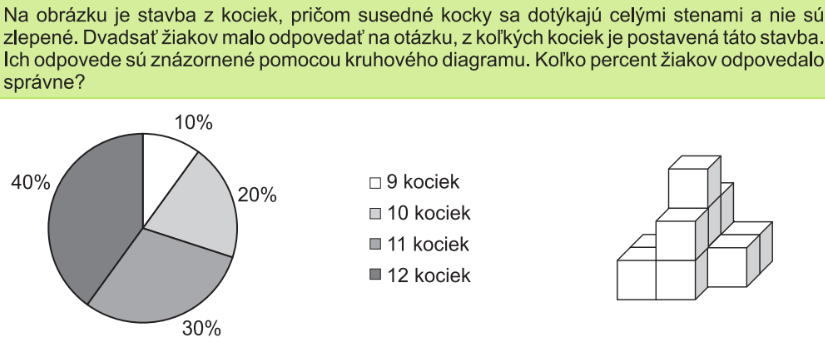
\includegraphics{assets/kocky.png}
	\end{center}
	
\end{example}

\begin{example}
	V prepravke sa nachádza niekoľko melónov. Počet melónov v prepravke označme $p$ a hmotnosť všetkých melónov v kilogramoch v prepravke označme $m$. Pomocou ktorého výpočtu vieme vypočítať preiemernú hmotnosť melónov v prepravke?
	
	\begin{enumerate}
		\item $m \div p$
		\item $m - p$
		\item $p \cdot m$
		\item $p \div m$
	\end{enumerate}
\end{example}

\begin{example}
	Je daná trojica čísel: 53; 56,9 a 55,4. Určte číslo, ktoré musíme odčítať od najmenšiaho z nich, aby aritmetický priemer bol 54.
\end{example}

\begin{center}
	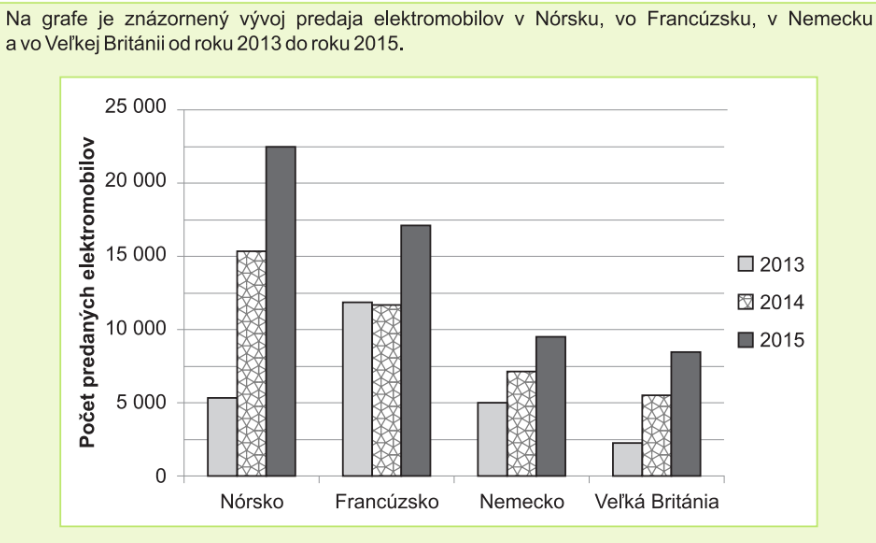
\includegraphics{assets/elektromobily_graf.png}
\end{center}

\begin{example}
	Koľko približne elektromobilov sa podľa grafu predalo vo Francúzsku v roku 2014?
	
	\begin{enumerate}
		\item 10 500
		\item 11 500
		\item 12 500
		\item 13 500
	\end{enumerate}
\end{example}

\begin{example}
	V ktorej krajine sa predalo iba v jednom z rokov 2013, 2014, 2015 viac elektromobilov, ako sa predalo v tom istom roku v Nórsku?
\end{example}

\begin{example}
	V stĺpcovom diagrame je znázornené umiestnenie Petra Sagana v jednotlivých etapách Tour de France v roku 2016. Všetkých etáp bolo spolu 21. Koľko percent predstavujú etapy, v ktorých sa umiestnil na 1. až 3. mieste? Výsledok zaokrúhli na celé číslo . 
	
	\begin{center}
		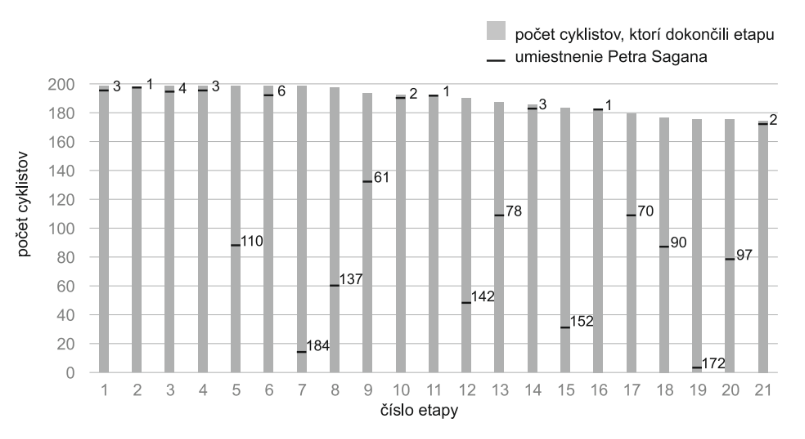
\includegraphics{assets/sagan_graf.png}
	\end{center}
\end{example}

\begin{example}
	Na hodine fyziky žiaci odhadovali objem smetného koša v triede. Na tabuli je záznam 20 odpovedí žiakov. Skutočný objem tohoto koša bol 12 litrov. O koľko litrov sa v priemere lýši odhad žiakov? 
	
	\begin{center}
		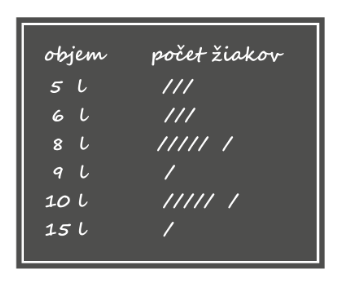
\includegraphics{assets/tabula.png}
	\end{center}
\end{example}

\begin{center}
	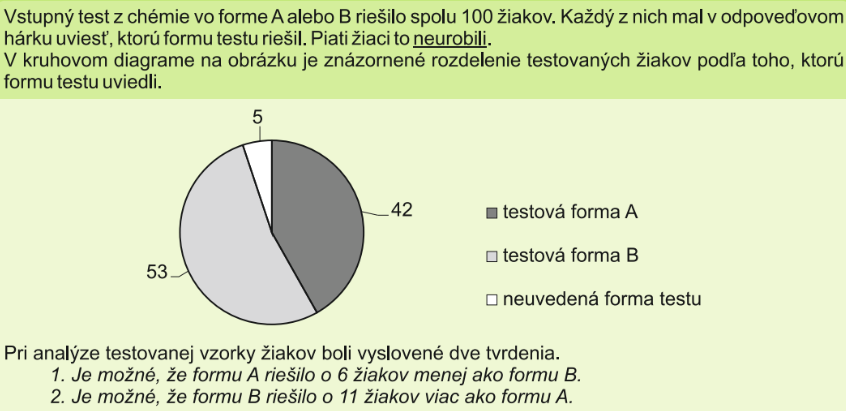
\includegraphics{assets/test_chemia.png}
\end{center}

\begin{example}
	Posúď pravdivosť týchto tvrdení a vyber správnu možnosť.
	
	\begin{enumerate}
		\item Len prvé tvrdenie je pravdivé.
		\item Len druhé tvrdenie je pravdivé.
		\item Obidve tvrdenia sú pravdivé.
		\item Ani jedno tvrdenie je pravdivé.
	\end{enumerate}
\end{example}

\begin{example}
	 \begin{center}
	 	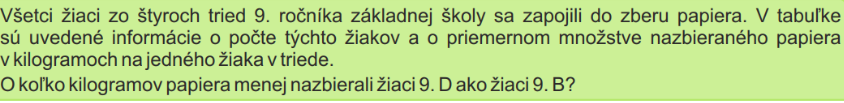
\includegraphics{assets/ziaci_zadanie.png}
	 	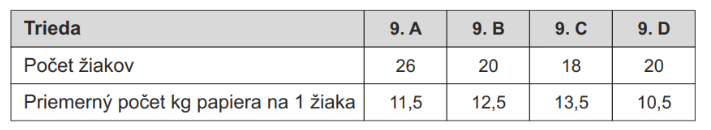
\includegraphics{assets/ziaci_graf.png}
	 \end{center}
\end{example}

\begin{example}
	\begin{center}
		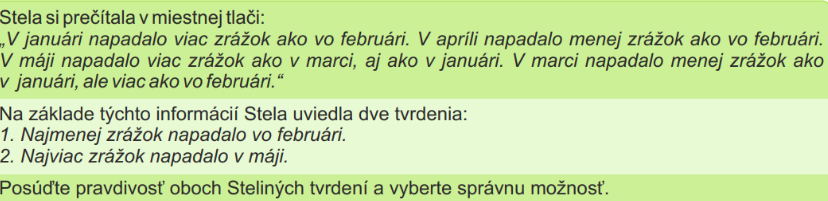
\includegraphics{assets/stela_zadanie.png}
	\end{center}
	
	\begin{enumerate}
		\item Obidve tvrdenia sú pravdivé.
		\item Len prvé tvrdenie pravdivé.
		\item Len druhé tvrdenie je pravdivé.
		\item Ani jedno tvrdenie nie je pravdivé.
	\end{enumerate}
\end{example}

\begin{center}
	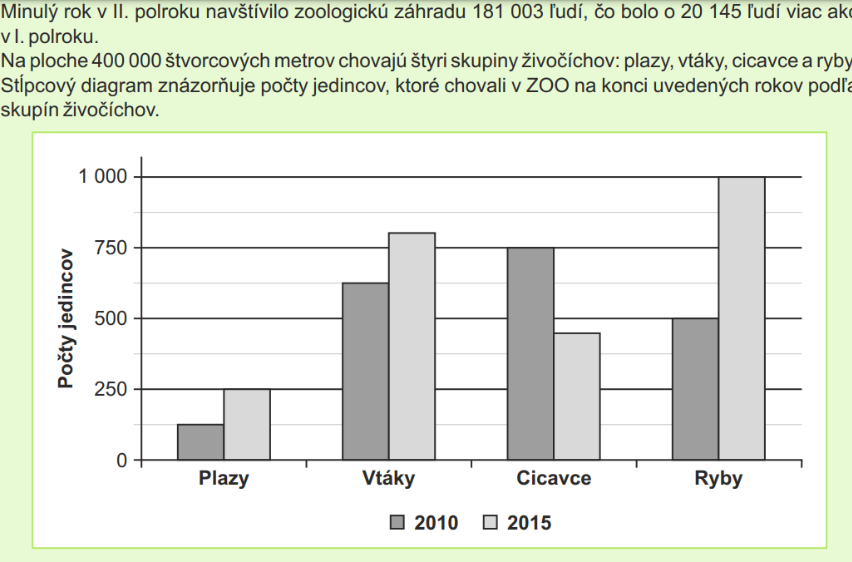
\includegraphics{assets/zoo_graf.png}
\end{center}

\begin{example}
	Koľko ľudí navštívilo túto zoologickú záhradu v minulom roku?
\end{example}

\begin{example}
	Koľko hektárov zaoberá v zoologickej záhrade plocha, na ktorej sú chované živočíchy?
\end{example}

\begin{example}
	Na základe údajov zobrazených v diagrame zisti, približne koľko jedincov  spolu chovali v tejto zoologickej záhrade na konci roku 2015.
\end{example}

\begin{example}
	V tabuľke sú uvedené ceny za výkopové práce v štyroch rôznych firmách. Vypočítajte, koľko eur je priemerná cena práce ručného výkopu za $m^3$ v uvedených firmách?
	
	\begin{center}
		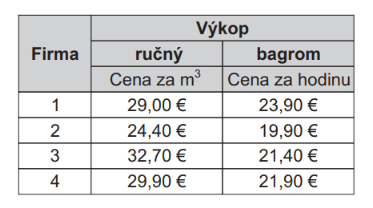
\includegraphics{assets/tab6.png}
	\end{center}
\end{example}

\begin{center}
	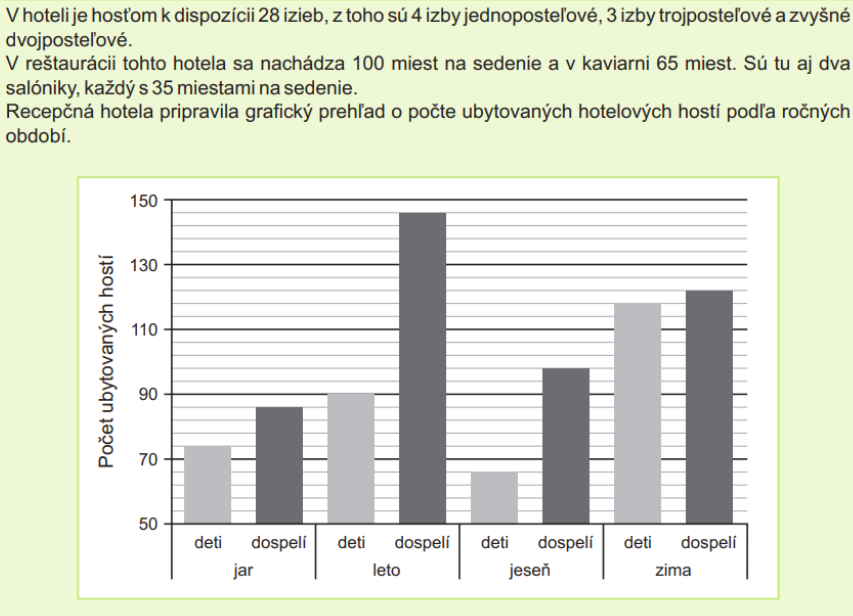
\includegraphics{assets/hotel_graf.png}
\end{center}

\begin{example}
	Na základe údajov uvedených v texte boli vyslovené nasledovné tvrdenia.
	
	\begin{itemize}
		\item Počet dvojposteľových izieb a počet všetkých izieb je v pomere 3:4.
		\item Počet detí a počet dospelých ubytovaných v zime je v pomere 23:24.
	\end{itemize}
	
	Posúďte pravdivosť týchto doch tvrdení a vyber správnu možnosť.
	
	\begin{enumerate}
		\item Obidve tvrdenia sú pravdivé.
		\item Obidve tvrdenia sú nepravdivé.
		\item Len prvé tvrdenie je pravdivé.
		\item Len druhé tvrdenie je pravdivé.
	\end{enumerate}
\end{example}

\begin{example}
	V ktorej možnosti kruhový diagram správne zobrazuje rozdelenie počtu miest na sedenie v tomto hoteli?
	
	\begin{center}
		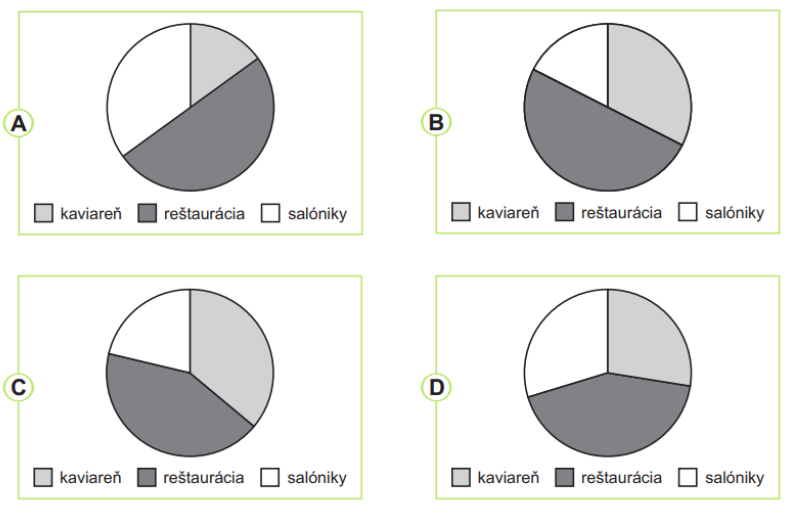
\includegraphics{assets/hotel_grafy.png}
	\end{center}
\end{example}

\begin{example}
	Ktorý brankár mal druhú najlepšiu percentuálnu úspešnosť?
	
	\begin{center}
		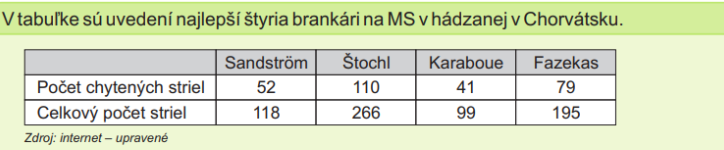
\includegraphics{assets/tab7.png}
	\end{center}
\end{example}

\begin{example}
	\begin{center}
		
\includegraphics{assets/kruhovy_diagram_zadanie.png}
		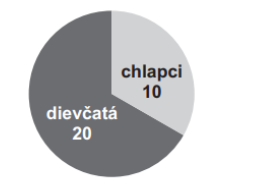
\includegraphics{assets/kruhovy_diagram.png}
	\end{center}
\end{example}

\begin{example}
	\begin{center}
		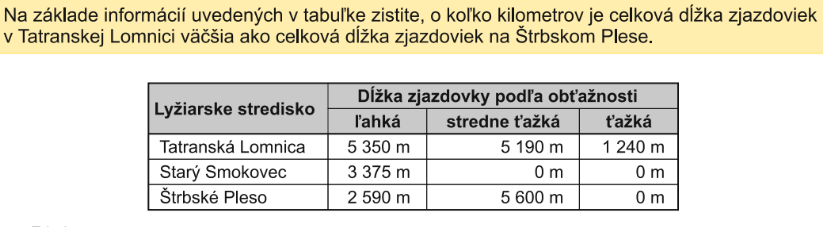
\includegraphics{assets/zjazdovky.png}
	\end{center}
\end{example}

\begin{center}
	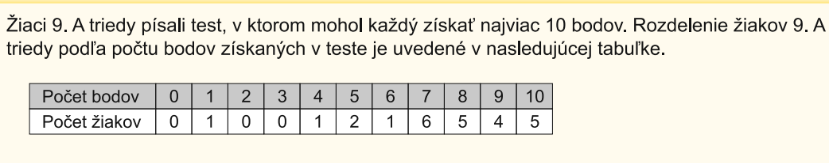
\includegraphics{assets/ziaci_tabulka.png}
\end{center}

\begin{example}
	Koľko žiakov 9.A triedy získalo v teste menej bodov, ako je priemerný počet bodov získaný všetkými žiakmi triedy?
\end{example}

\begin{example}
	Adam získal 6 bodov. Údaje uvedené v tabuľke spracoval do stĺpcového diagramu. Stĺpec znázorňujúci počet žiakov s 10 bodmi mal výšku 7,5 cm. Vypočítaj, koľko centimetrov vysoký bol stĺpec znázorňujúci počet žiakov so 7 bodmi.
	
	\begin{center}
		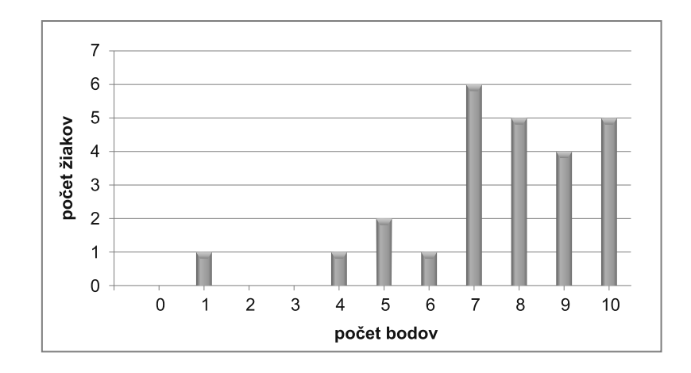
\includegraphics{assets/stlpce.png}
	\end{center}
\end{example}

\begin{center}
	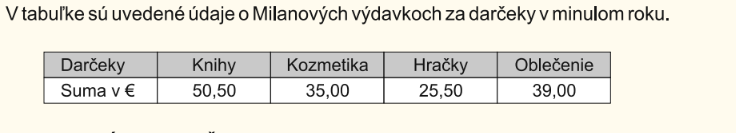
\includegraphics{assets/tab8.png}
\end{center}

\begin{example}
	Ktorý kruhový diagram správne zobrazuje  rozdelenie Milanových výdavkov za darčeky?
	
	\begin{center}
		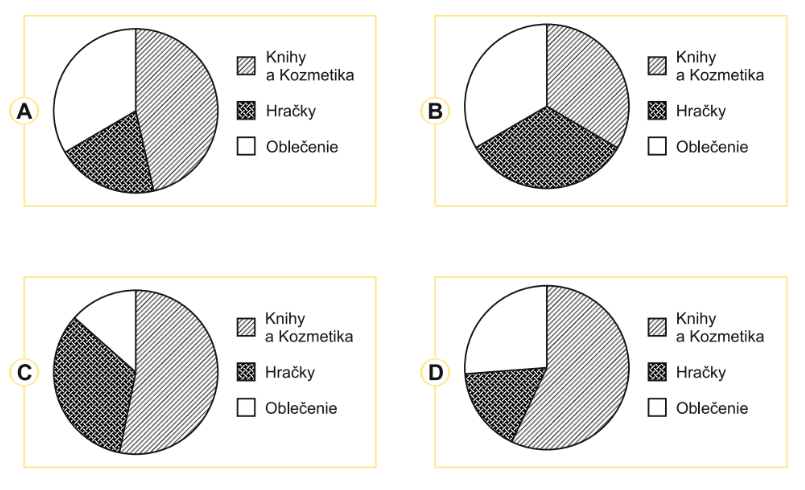
\includegraphics{assets/kruhove_diagramy.png}
	\end{center}
\end{example}

\begin{example}
	Tento rok Milan plánuje znížiť výdavky za darčeky o 15\% oproti minulému roku. Koľko eur plánuje Milan minúť na darčeky tento rok?
\end{example}

\begin{example}
	Graf znázorňuje rozdelenie poľnohospodárskej pôdy s rozlohou 48 hektárov, ne ktorej boli vysiate štyri plodiny. Na koľkých ároch bola vysiata repa?
	
	\begin{center}
		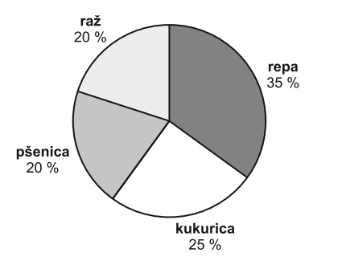
\includegraphics{assets/kruhovy_diagram2.png}
	\end{center}
\end{example}

\begin{center}
	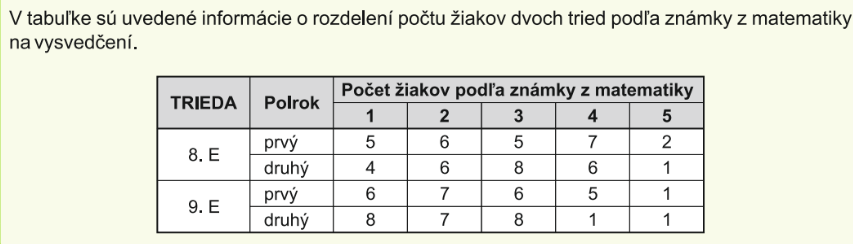
\includegraphics{assets/tab9.png}
\end{center}

\begin{example}
	Na základe informácií uvedených v tabuľke vypočítaj priemer známok z matematiky žiakov 8. E treidy ny vysvedčení v druhom polroku. Výseldok uveď v tvare desatinného čísla s presnoťou na stotiny.
\end{example}

\begin{example}
	Graf znázorňuje informácie uvedené v jednom z riadkov z predchádzajúcej tabuľky.
	
	\begin{center}
		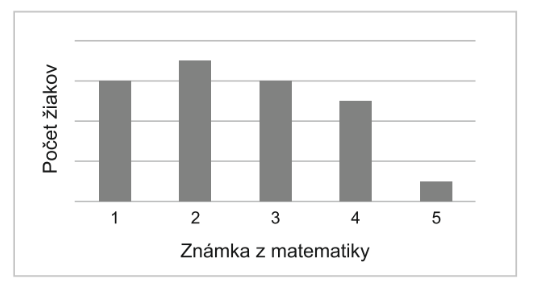
\includegraphics{assets/stlpce2.png}
	\end{center}
	
	V grafe je znázornené rozdelenie počtu žiakov podľa známky z matematiky z triedy:
	
	\begin{enumerate}
		\item 9. E v druhom polroku
		\item 9. E v prvom polroku
		\item 8. E v druhom polroku
		\item 8. E v prvom polroku
	\end{enumerate}
\end{example}